\documentclass[a4paper,12pt]{report}
%\documentclass[twoside]{article}
%\usepackage{extsizes}
\usepackage{cmap}
\usepackage[utf8]{inputenc} %Кодировка файла 
\usepackage[T2A]{fontenc} %корректное отображение русских шрифтов
\usepackage[english, russian]{babel} %переносы слов
\usepackage{fancyvrb}
\usepackage{lmodern}

%for lcov
\usepackage{lscape} %landspace
\usepackage{float}
\usepackage{tabu}
\usepackage{booktabs}
%\usepackage{xcolor}
%\definecolor{coverage_Hi}{rgb}{0, 1, 0}
%\definecolor{coverage_Med}{rgb}{1, 1, 0}
%\definecolor{coverage_Lo}{rgb}{1, 0, 0}
%\definecolor{cov_cov}{rgb}{0.9,0.9,1}
%\definecolor{cov_diff}{rgb}{1,1,0.5}
%\definecolor{cov_nocov}{rgb}{1,0.5,0.5}
%\definecolor{cov_nop}{rgb}{0.95,0.95,0.95}
\usepackage{listings}
\usepackage{picture}

\usepackage{graphicx}

%\linespread{1.3}
\renewcommand{\rmdefault}{ftm}
%\frenchspacing

%TimeNewRoman
%\usepackage{fontspec}
%\setmainfont[Mapping=tex-text]{Times New Roman}

%Поля
\usepackage{geometry}
\geometry{left=3cm}
\geometry{right=1.5cm}
\geometry{top=2.4cm}
\geometry{bottom=2.4cm}

\usepackage{verbatim}
\usepackage{spverbatim}
\renewenvironment{lstlisting}{\spverbatim}{\endverbatim}

%\renewcommand{\labelenumii}{\arabic{enumi}.\arabic{enumii}.} %стиль нумерованных списокв

\usepackage[parentracker=true,%
  backend=biber,%
  language=auto,%
  autolang=other,%
  %citestyle=gost-numeric,%
  defernumbers=true,%
  %bibstyle=gost-numeric,%
]{biblatex}
\addbibresource{bibliography.bib}

%НАСТРОЙКИ ДЛЯ DOXYGEN

\usepackage{longtable}

\usepackage{fixltx2e}
\usepackage{calc}
\usepackage{doxygen}
\usepackage[export]{adjustbox} % also loads graphicx
\usepackage{makeidx}
\usepackage{multicol}
\usepackage{multirow}
\PassOptionsToPackage{warn}{textcomp}
\usepackage{textcomp}
\usepackage[nointegrals]{wasysym}
\usepackage[table]{xcolor}



% Font selection
%\usepackage[T1]{fontenc}
\usepackage[scaled=.90]{helvet}
\usepackage{courier}
\usepackage{amssymb}
\usepackage{sectsty}
\renewcommand{\familydefault}{\sfdefault}
\allsectionsfont{%
  \fontseries{bc}\selectfont%
  \color{darkgray}%
}
\renewcommand{\DoxyLabelFont}{%
  \fontseries{bc}\selectfont%
  \color{darkgray}%
}
\newcommand{\+}{\discretionary{\mbox{\scriptsize$\hookleftarrow$}}{}{}}

% Page & text layout
%\usepackage{geometry}
%\geometry{%
%  a4paper,%
%  top=2.5cm,%
%  bottom=2.5cm,%
%  left=2.5cm,%
%  right=2.5cm%
%}
\tolerance=750
\hfuzz=15pt
\hbadness=750
\setlength{\emergencystretch}{15pt}
\setlength{\parindent}{0cm}
\setlength{\parskip}{3ex plus 2ex minus 2ex}
\makeatletter
\renewcommand{\paragraph}{%
  \@startsection{paragraph}{4}{0ex}{-1.0ex}{1.0ex}{%
    \normalfont\normalsize\bfseries\SS@parafont%
  }%
}
\renewcommand{\subparagraph}{%
  \@startsection{subparagraph}{5}{0ex}{-1.0ex}{1.0ex}{%
    \normalfont\normalsize\bfseries\SS@subparafont%
  }%
}
\makeatother

% Headers & footers
\usepackage{fancyhdr}
\pagestyle{fancyplain}
\fancyhead[LE]{\fancyplain{}{\bfseries\thepage}}
\fancyhead[CE]{\fancyplain{}{}}
\fancyhead[RE]{\fancyplain{}{\bfseries\leftmark}}
\fancyhead[LO]{\fancyplain{}{\bfseries\rightmark}}
\fancyhead[CO]{\fancyplain{}{}}
\fancyhead[RO]{\fancyplain{}{\bfseries\thepage}}
\fancyfoot[LE]{\fancyplain{}{}}
\fancyfoot[CE]{\fancyplain{}{}}
\fancyfoot[RE]{\fancyplain{}{\bfseries\scriptsize Овчинников Владислав Александрович }}
\fancyfoot[LO]{\fancyplain{}{\bfseries\scriptsize Овчинников Владислав Александрович }}
\fancyfoot[CO]{\fancyplain{}{}}
\fancyfoot[RO]{\fancyplain{}{}}
\renewcommand{\footrulewidth}{0.4pt}
\renewcommand{\sectionmark}[1]{%
  \markright{\thesection\ #1}%
}

% Indices & bibliography
%\usepackage{natbib}
\usepackage[titles]{tocloft}
\setcounter{tocdepth}{3}
\setcounter{secnumdepth}{5}
\makeindex

% Hyperlinks (required, but should be loaded last)
\usepackage{ifpdf}
\ifpdf
  \usepackage[pdftex,pagebackref=false]{hyperref}
\else
  \usepackage[ps2pdf,pagebackref=false]{hyperref}
\fi
\hypersetup{%
  colorlinks=true,%
  linkcolor=blue,%
  citecolor=blue,%
  unicode%
}

% Custom commands
\newcommand{\clearemptydoublepage}{%
  \newpage{\pagestyle{empty}\cleardoublepage}%
}

\usepackage{caption}
\captionsetup{labelsep=space,justification=centering,font={bf},singlelinecheck=off,skip=4pt,position=top}



\usepackage[pdf]{graphviz}

\title{Разработка SMTP-клиента как части MTA. Вариант \textnumero 26}
\author{(Студент группы ИУ7-33М: Овчинников Владислав Александрович.)}

\begin{document}
	\maketitle

	\tableofcontents

	\addcontentsline{toc}{chapter}{Введение}
	\chapter*{Введение}
	Практически каждое вычислительное устройство должно обмениваться данными с другими вычислительными устройствами, среди которых можно выделить - компьютеры, серверы, маршрутизаторы и многие другие устройства, которые требуют данные извне. Система, обеспечивающая обмен между такими устройствами называется компьютерной сетью. Для функционирования компьютерных сетей используются сетевые протоколы.

	Сетевой протокол - это набор программно-реализованных правил общения компьютеров, подключенных к сети. В настоящее время стандартом стало использование стека протоколов TCP/IP.
	
	В стеке протоколов TCP/IP были выделены четыре следующих уровня передачи информации между процессами:
	
	\begin{itemize}
		\item Канальный уровень (Ethernet, PPP, HDLC) -- предназначен для передачи данных между сетевыми адаптерами в одном сегменте сети. Также может использоваться для обнаружения и, возможно, исправления ошибок, возникших на физическом уровне.
		\item Сетевой уровень (IP) -- предназначен для передачи данных между компьютерами в разных сегментах сети. Основная цель: определение пути передачи данных. Отвечает за трансляцию логических адресов в физические. 
		\item Транспортный уровень (TCP, UDP) -- предназначен для передачи данных между процессами на разных компьютерах. При этом неважно, какие данные передаются, т.е. представляет сам механизм передачи.
		\item Прикладной уровень (HTTP, SMTP) -- обеспечивает взаимодействие сети и пользователя, разрешает приложениям пользователя иметь доступ к сетевым службам, таким как обработчик запросов к базам данных, доступ к файлам, пересылке электронной почты, просмотру веб-страниц и т.д.
	\end{itemize}

	В данной курсовой работе рассматривается разработка SMTP-клиента. Simple Mail Transfer Protocol (SMTP) - это широко используемый сетевой протокол, предназначенный для передачи электронной почты в сетях TCP/IP. SMTP впервые был описан в RFC 821. Последнее обновление в RFC 5321 включает масштабируемое расширение - ESMTP. Протокол SMTP предназначен для передачи исходящей почты с использованием порта TCP 25.

	Целью курсовой работы является реализация SMTP-клиента (как части MTA), обеспечивающего удаленную доставку и поддерживающего очереди сообщении. Вариант лабораторной работы подразумевает реализацию многопоточного SMTP-клиента с использованием вызова pselect.

	\chapter{Аналитический раздел}
	\section{Основные понятия протокола SMTP}
	В рамках курсовой работы требовалось разработать SMTP-клиент как часть MTA. Перед разработкой архитектуры был проведен анализ предметной области, связанной с решением поставленной задачи. Был рассмотрен SMTP-протокол, MTA, DNS.

	SMTP (Simple Mail Transfer Protocol) - протокол передачи сообщений с компьютера на почтовый сервер для доставки конечному получателю. Этот протокол обеспечивает перенаправление почтовых сообщений с помощью записей типа MX (или записей программы обмена электронной почтой) и записей типа A (или записей сервера в системе DNS), форматирование почтовых сообщений и установление сеансов между почтовыми клиентами и почтовыми серверами. В протоколе SMTP в качестве транспортного протокола обычно используется TCP, но могут применяться и другие протоколы, как определено в документе RFC 821.

	Обмен данными в рамках SMTP строится по принципу двусторонней связи, которая устанавливается между отправителем и получаетелем почтового сообщения. При этом отправитель инициирует соединение и посылает запросы на обслуживание, а получатель - отвечает на эти запросы. Фактически, отправитель выступает в роли клиента, а получатель - сервера. Канал связи устанавливается непосредственно между отправителем и получателем сообщения.

	Протокол SMTP не несет никакой ответственности за прием почты. В спецификации этого протокола не определены способы настройки почтовых ящиков для отдельных пользователей, а также не упоминаются какие-либо иные задачи (такие как аутентификация), которые должны быть решены при приеме электронной почты. В этой спецификации просто указано, как должна осуществляться передача электронной почты от отправителя к получателю.

	Основная задача протокола SMTP заключается в том, чтобы обеспечивать передачу электронных сообщений. Для работы через протокол SMTP клиент создает TCP-соединение с сервером через порт 25. Затем клиент и SMTP-сервер обмениваются информацией пока соединение не будет закрыто или прервано. Основной процедурой в SMTP является передача почты (Mail Procedure). Далее идут процедуры Mail Forwarding, проверка имен почтового ящика и вывод списка почтовых групп. Самой первой процедурой является открытие канала передачи, а последней - его закрытие.

	MTA (Mail Transfer Agent) - самостоятельное, минимально достаточное для приема и отправки электронной почты программное обеспечение. Важнейшей частью почтового сервера является MTA (Mail Transfer Agent - агент пересылки почты), в задачи которого входит прием и передача почты.

	MTA работает по протоколу SMTP и его одного достаточно для создания системы электронной почты. Работа MTA совмещает в себе одновременно функции внешней и локальной доставки и получения почты. MTA, получая письмо, помещает его в почтовый ящик пользователя на своем сервере, к которому последний должен получить доступ.

	MDA (Mail Delivery Agent) - это агент доставки почты, его задача по запросу почтового клиента передать ему почту из почтового ящика на сервере. MDA может работать по протоколам POP3 (Post Office Protocol v3) или IMAP (Internet Message Access Protocol), в ряде случаев для "общения" почтового клиента и агента доставки могут применяться собственные протоколы, обладающие расширенной функциональностью, например MAPI (Messaging Application Programming Interface) в Exchange Server.

	MTA (Mail Transfer Agent - агент пересылки почты) - отвечает за пересылку почты между почтовыми серверами, как правило, первый MTA в цепочки получает сообщения от MUA (почтовый агент пользователя), последний MTA передает сообщение к MDA.

	MUA (Mail User Agent) - программа, обеспечивающая пользовательский интерфейс, отображающая полученные письма и предоставляющая возможность отвечать, создавать и перенаправлять письма.

	Общение с SMTP сервером ведется при помощи команд. Команды SMTP указывают, какую операцию хочет произвести клиент. Команды состоят из ключевых слов, за которыми следует один или более параметров, Ключевое слово состоит из 4-х символов и разделено от аргумента одним или несколькими пробелами. Каждая команда заканчивается символами CRLF. Обычный ответ SMTP-сервера состоит из номера ответа, за которым через пробел следует дополнительный текст. Номер ответа служит индикатором состояния сервера.

	\begin{itemize}
		\item EHLO -- данная команда используется для начала диалога клиента с сервером и получения расширений ESMTP, которые доступны для данного сервера (устаревшая - HELO).
		\item HELO -- устаревшая стандартная команда SMTP для начала диалога клиента с сервером (не позволяет получать расширения ESMTP).
		\item MAIL -- определяет отправителя сообщения, используется для ответных сообщений в случае невозможности доставки письма. Для каждого письма команда MAIL должна быть выполнена только один раз.
		\item RCPT -- определяет получателей сообщения. Доставка сообщения возможна тогда, когда указан хотя бы один доступный адрес получателя. Команда RCPT принимает в качестве аргумента только один адрес. Если нужно послать письмо большему числу адресатов, то команду RCPT следует повторять для каждого.
		\item DATA -- определяет начало сообщения. С помощью этой команды серверу передается текст сообщения, состоящий из заголовка и отделенного от него пустой строкой тела сообщения. Команда DATA может быть выполнена только после успешного выполнения хотя бы одной команды RCPT.
		\item QUIT -- остановка сеанса SMTP. Клиент заканчивает диалог с сервером. Сервер посылает подтверждение и закрывает соединение. Получив это подтверждение, клиент тоже прекращает связь.
		\item HELP -- запрашивает список команд. Если команда HELP вызывается без параметров, сервер посылает клиенту список доступных команд. Если в качестве параметра передано название команды, то клиенту посылается описание этой команды.
		\item VRFY -- проверяет имя пользователя системы. Используется для проверки наличия указанного в качестве аргумента почтового ящика. В ответ сервер посылает информацию о владельце ящика или сообщение об ошибке, свидетельствующее о том, что указанный ящик не существует.
		\item EXPN -- используется для получения адресов, внесенных в список рассылки.
		\item NOOP -- в ответ на данную команду сервер посылает подтверждение выполнения. Никаких действий на сервере не производится, параметры команды игнорируются.
		\item RSET -- сброс SMTP-соединения. Данная команда аннулирует все переданные до нее на сервер данные. Процесс передачи сообщения следует начать заново с выполнения команды EHLO (HELO).
		\item TURN -- смена направления передачи. 
	\end{itemize}

	\section{SMTP-сессия}
	
	По протоколу SMTP отправитель письма связывается с получателем при помощи командной строки и специальных каналов, роль которых обычно выполняет TCP-соединение. Любая SMTP-сессия состоит из двух ведующих компонентов: команд от клиента и соответствующих им ответов сервера. При открытой сессии обе этих составляющих обмениваются ее параметрами. Подобный обмен может включать как ноль, так и больше SMTP-операций (транзакций).

	Классическая SMTP-сессия включает в себя следующие этапы:
	\begin{enumerate}
		\item Инициирование соединения. Клиент создает соединение с сервером. Сервер отвечает клиенту сообщением с кодом отклика 220 в случае готовности для продолжения работы или с кодом отклика 554 в случае отказа в открытии SMTP-сессии.
		\item Инициирование работы с клиентом. Клиент передает команду EHLO (HELO). Сервер отправляет сообщение с кодом отклика 250. Если была отправлена команда EHLO, сервер также в сообщении возвращает список расширений, который он поддерживает. Сервер также может вернуть сообщение с кодом отклика 501, если не было передано в аргументах команды имя клиента (может быть любым, но обычно проверяется для борьбы со спамом с помощью PTR-записи).
		\item SMTP-транзакция (в процессе SMTP-сессии их может быть несколько).
		\item Завершение сессии. Если клиент желает завершить работу с сервером, то он посылает команду QUIT, на которую сервер отвечает сообщением с кодом отклика 221 и закрывает соединение. По данной команде можно определить, что клиент также должен освободить ресурсы под выделенное соединение.
	\end{enumerate}

	Любая SMTP-транзакция представляет собой три последовательные этапа команда/ответ:
	\begin{enumerate}
		\item MAIL from. Определяет обратный адрес. Эта переменная необходима для возвращенных писем. Сервер в случае принятия данных отвечает сообщением с кодом отклика 250 в случае успеха. Но может также ответить с кодом отклика 501 (синтаксическая ошибка). 
		\item RCPT to. Определяет получателя текущего текстового сообщения. Команда может использоваться несколько раз, в зависимости от количества получателей. Сервер в случае принятия данных отвечает сообщением с кодом отклика 250 в случае успеха. Сообщение с кодом отклика 501 возвращается в случае синтаксической ошибки, а с кодом отклика 503 в случае невозможности принятия данных на данном этапе, с кодом отклика 550 - если пользователь не найден на сервере.
		\item DATA. Определяется для последовательной отправки текстового сообщения. Включает в себя непосредственно содержимое письма, в отличие от оболочки. "DATA" несет в себе информацию о заголовке и теле сообщения (они разделяются пустой строкой). Ответ от сервера при передаче происходит в два этапа: на первом от отвечает конкретно на команду "DATA" (уведомление о готовности принять текстовое сообщения), а на втором - о принятии или отклонении всего письма в конце последовательности данных. После выполнения команды DATA сервер возвращает в случае успеха сообщение с кодом 354, что означает, что сервер готов принимать содержимое письма, на все последующие данные сервер не будет отвечать до того момента, пока не встретит последовательность из <CRLF>.<CRLF>. В случае успеха получения сервером всего текста письма он отвечает сообщением с кодом отклика 250.
	\end{enumerate}

	Стоит отметить, что SMTP-сервер может разоравать SMTP-сессию в случае истечения времени ожидания. Тогда он вернет сообщение с кодом отклика 421, что свидетельствует о том, что сервер разорвал соединение, и клиент должен освободить ресурсы, выделенные под SMTP-сессию.  

	Любой SMTP-сервер выполняет несколько функций. Одной из них является проверка правильности настроек и выдача разрешения компьютеру, который пытается отправить электронное письма. Другая функция состоит в отправке исходящих писем на указанный адрес с последующей проверкой доставки. В качестве задачи, которую необходимо решить в рамках данной курсовой работы, является реализация функции отправки исходящих писем, т.е. реализация SMTP-клиента как части MTA.


	\section{Архитектура взаимодействия клиента с сервером}

        В процессе курсовой работы требовалось разработать SMTP-клиент как часть MTA для организации удаленной доставки письма после его получения и записи в каталог MAILDIR. Организация удаленной доставки может быть обеспечена следующим образом:
	\begin{enumerate}
		\item Определение имени сервера по пути сервера, в каталоге в MAILDIR которого находятся письма, для определения того, куда необходимо передавать доступные для удаленной доставки письма.
		\item Открытие необходимого соединения SMTP-клиента c SMTP-сервером для последующей сессии.
		\item Начало сессии и инициирование общения с ним c помощью команды HELO.
		\item Считывание данных письма и последующий анализ дополнительных заголовков необходимых для последующей отправки.
		\item Передача адреса почтового ящика отправителя в MAIL. Данный адрес считывается из дополнительных заголовков письма.
		\item Попытка передачи всех возможных адресов получателей, которые были считаны из текста файла, содержащего текст письма.
		\item Проверка корректности переданных данных с помощью команды DATA, так как в случае успеха данная команда вернет сообщение с кодом отклика 354.
		\item Передача текста письма.
		\item Передача флага текста письма и получение сообщения с откликом.
		\item В случае успеха файл доставленного сообщения может быть удален (и удаляется). В случае неудачи, на каком-то из шагов удаление сообщения происходит при анализе ошибки. Если код ошибки 4xx, то в большинстве случаев это ошибка не связана с работой сервера и, желательно, повторить отправку. Если же код ошибки 5xx, то в большинстве случаев это означает ошибку, которую совершает клиент и сервер в любом случае не примет данное сообщение, следует удалить файл с текстом письма.
		\item Если есть еще сообщения, то можем продолжить отправку, иначе закрыть соединение и завершить сессию до появления новых сообщений.
	\end{enumerate}
	
	\begin{figure}[H]
		\centering
		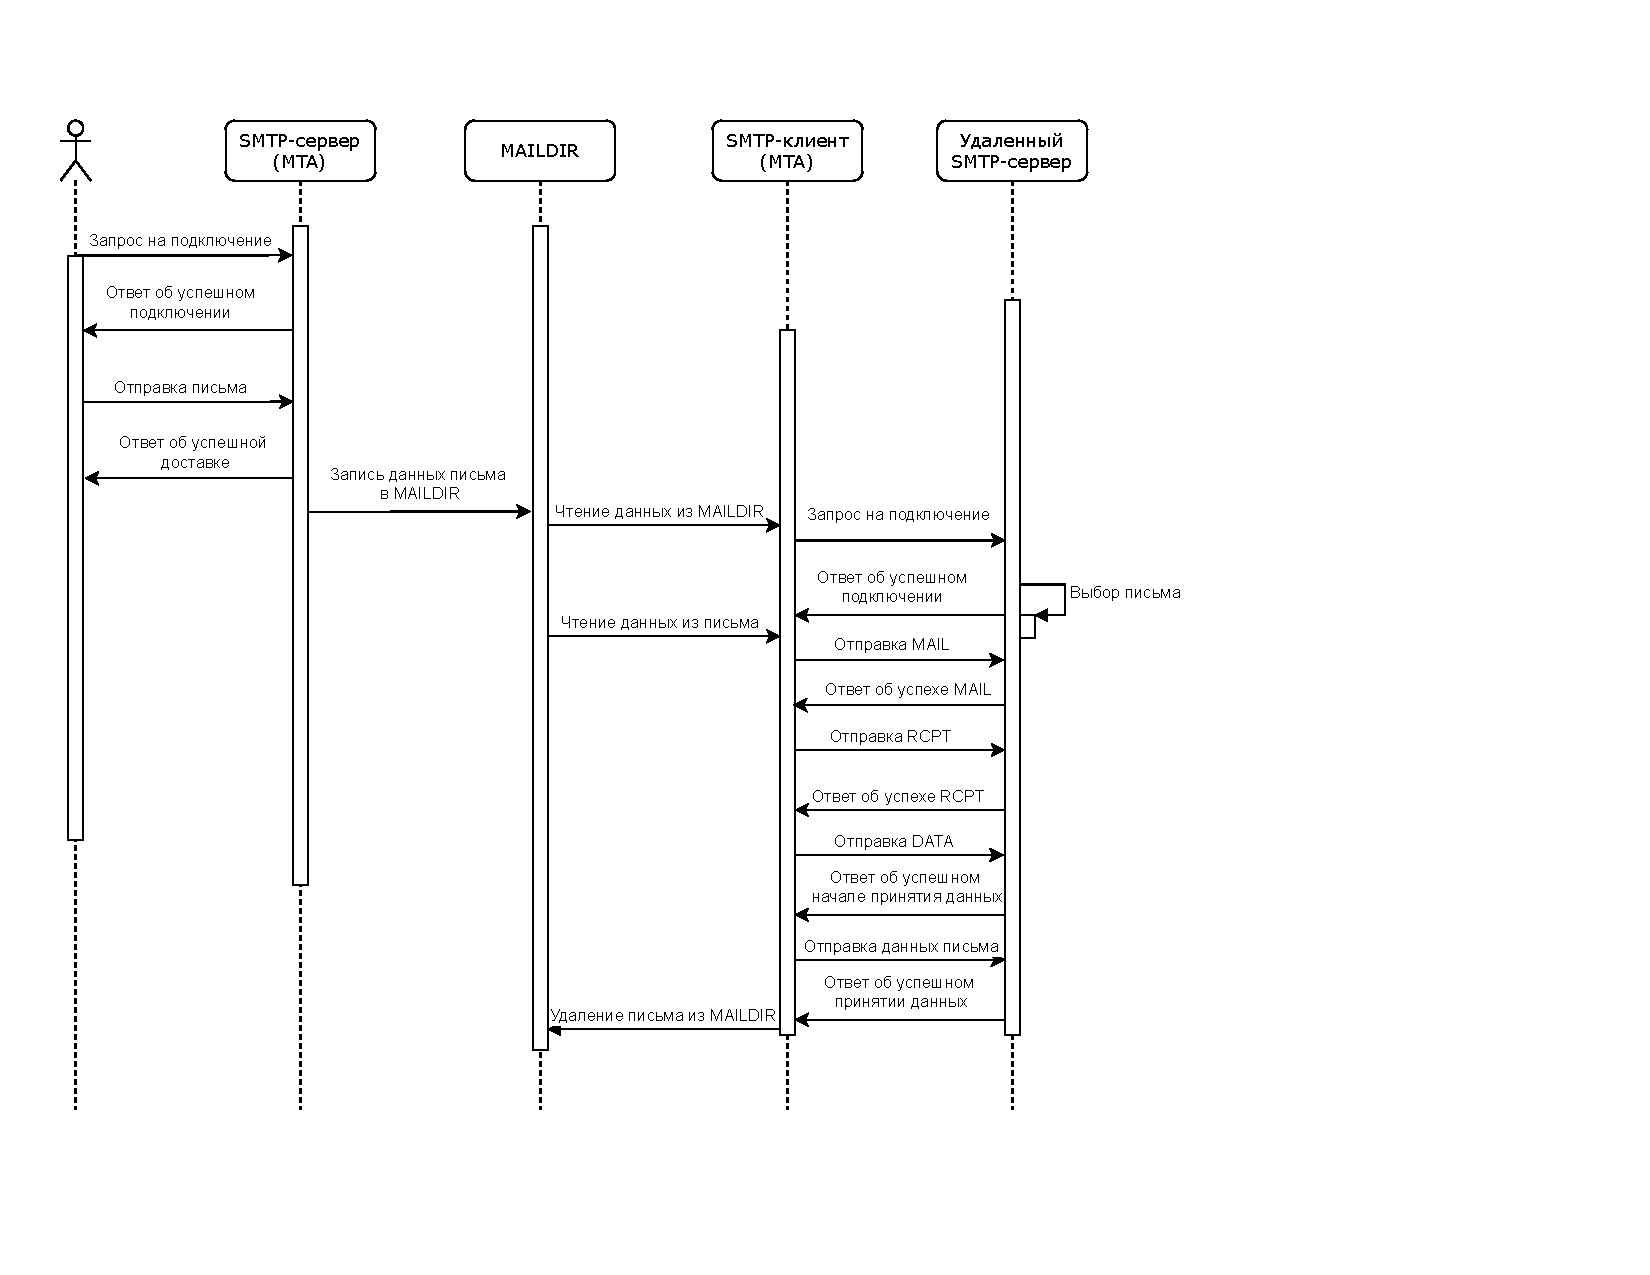
\includegraphics[width=1.5\textwidth]{./resource/diagram_seq.pdf}
		\caption{Диграмма последовательности взаимодействия клиента с сервером} 
		\label{fig:EventLoopSequence}
	\end{figure}

	От SMTP-клиента как части MTA требуется способность работать с множеством исходящих подключений к удаленным SMTP-серверам. Для решения данной проблемы можно воспользоваться несколькими способами:
	\begin{enumerate}
		\item Один клиент - один поток (процесс). Одним из решений задачи обслуживания нескольких исходящих подключений является использование многопоточных возможностей ОС: можно создать отдельный поток для обслуживания одного клиента. Данный многопоточный подход имеет ряд недостатков. Создание нового потока - сравнительно затратная операция для ОС. В периоды пиковой нагрузки на сервер большое число одновременно запущенных потоков может исчерпать ресурсы системы, а непрерывное создание, переключение и завершение потоков только ухудшит ситуацию.
		\item Пул потоков. Для решения проблемы траты ресурсов часто применяют пул заранее созданных потоков ограниченного размера, что в принципе при огромном количестве одновременных подключений не решает проблему.
		\item Мультиплексирование при работе с сокетами: select, poll, pselect, epoll. Если потоки или процессы сервера большую часть времени проводят в ожидании сообщений от клиента или вспомогательных служб, а не занимаются сложными вычислениями, пользы от многопоточности будет мало. Альтернативой в этом случае является ожидание событий на множестве сокетов в одном потоке исполнения. Для этого используются функции select, poll, pselect или epoll. Общая идея такова: в функцию передается массив дескрипторов сокетов. Функция блокирует выполнение до тех пор, пока один из сокетов в массиве не станет доступен для неблокирующего чтения (т.е. поступили новые данные или новое соединение) или записи (освободился буфер отправки), либо пока не истечет указанный таймаут. Все взаимодействие с сокетами осуществляется в одном потоке исполнения, что снимает необходимость синхронизации доступа к разделяемым ресурсам.
	\end{enumerate}

	В процессе выполнения курсовой работы требовалось разработать SMTP-клиент таким образом, чтобы он обрабатывал несколько исходящих соединений в одном потоке исполнения и при этом поддерживал многопоточную обработку. Требуется воспользоваться вызовом pselect.

	Вызов pselect почти ничем не отличается от вызова select. Вызов pselect имеет аргумент, который содержит набор сигналов, которые ядро должно разблокировать (то есть удалить из маски сигналов, вызывающего потока) на время, пока вызывающий поток заблокирован в вызове pselect. В остальном он полностью схож с вызовом select, который имеет ряд недостатков:

	\begin{itemize}
		\item Вызов select (pselect) модифицирует передаваемые ему структуры fdsets, так что ни одну из них нельзя переиспользовать. Даже если, например, получив порцию данных, а требуется получить еще, структуры fdsets необходимо переинициализировать. Ну или копировать из заранее сохраненного бэкапа.
		\item Для выяснения того, какой именно дескриптор сгенерировал событие, требуется вручную опросить их все.
		\item Максимальное количество одновременно наблюдаемых дескрипторов ограниченно константной и может быть ограничено в 1024 дескриптора.
		\item Невозможно работать с дескрипторами из наблюдаемого набора из другого потока.
	\end{itemize}

	Исходя из вышеперечисленных недостатков можно сделать вывод, что следует учесть в проектировании SMTP-клиента максимальное количество допустимых дескрипторов.

 	\chapter{Конструкторский раздел}

 	\section{Разработка SMTP-клиента}
    
    	\begin{figure}[h]
		\centering
		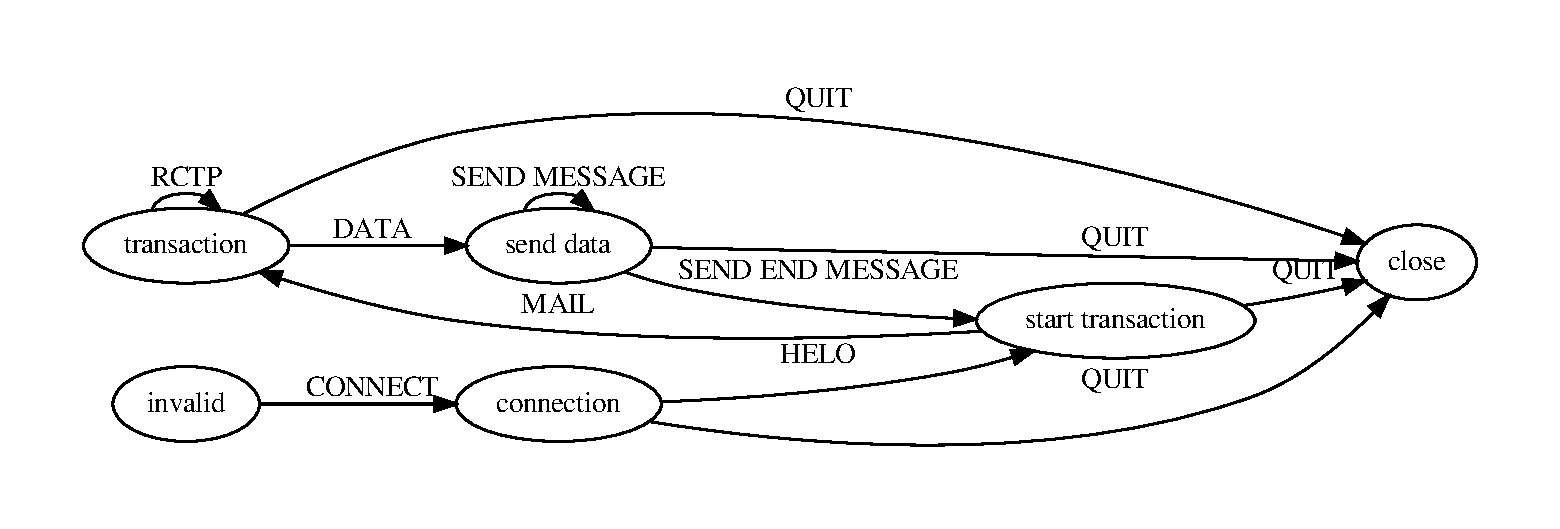
\includegraphics[width=\textwidth]{./include/smtp_states.pdf}
		\caption{Конечный автомат протокола SMTP для клиента}
		\label{fig:smtp_states}
	\end{figure}
     
	Каждая SMTP-сессия представляет собой совокупность состояний (т.е. что требуется сделать в данный момент или что будет требоваться далее) и множество переходов между этими состояниями (в данном случае это определяется с помощью команд при работе с SMTP-сервером). В связи с этим допустимо построить конечный автомат для протокола SMTP.

	Конечный автомат - это математическая абстракция, которая состоит из трех основных элементов: множества внутренних состояний, множества входных сигналов, которые определяют переход из текущего состояния в следующее, множество конечных состояний, при переходе в которые автомат завершает работу.

	Конечный автомат, представленный на рисунке \ref{fig:smtp_states}, описывает состояния, изображенные в виде овалов, и переходы, изображенные на рисунке в виде дуг графа. Данный конечный автомат построен при помощи утилиты \textit{autofsm}.

	Были выделены следующие состояния конечного автомата:
	\begin{enumerate}
		\item invalid - данное состояние определяет, что клиент находится в невалидном для обмена данными состоянии, т.е. соединение с сервером не установлено, сокет не был открыт.
		\item connection - данное состояние определяет, что клиент успешно подключился к серверу, и может выполнять доступные ему команды, в данном случае SMTP-клиент может выполнить только 2 команды HELO и QUIT. Выполнение команды QUIT происходит только тогда, когда SMTP-сервер ответил клиенту сообщением с кодом отклика, означающего ошибку, тогда клиент инициирует закрытие сокета.
		\item start transaction - после выполнения команды HELO, когда клиент находится в состоянии connection, он переходит в состояние start transaction, которое обозначает, что можно начинать выполнять SMTP-транзакцию (т.е. подготовку для передачи данных и непосредственно передачу письма SMTP-серверу). Подготовка к передаче данных осуществляется путем выполнения команд MAIL, RCTP, DATA. Переход на следующую стадию подготовки к передаче производится путем выполнения команды MAIL, если сервер при ее выполнении возвращает сообщение с кодом отклика об успехе, иначе на данном этапе клиент произведен завершение сессии путем перехода в состояние close с помощью команды QUIT.
		\item transaction - данное состояние определяет то, что MAIL прошел успешно и теперь требуется отправить адреса электронных ящиков получателей сообщения. Производится это путем выполнения команды RCTP. Выполнение команды QUIT производится на данной стадии при возникновении критических ошибок, которые вернул сервер в сообщении (например, таймаут или синтаксическая ошибка в команде). В случае сообщения об отсутствии адреса электронного ящика на сервере клиент не прекратит попытки отправки по причине того, что другие электронные ящики могут присутствовать на сервер и это сообщение будет доставлено кому-нибудь. Переход из данного состояние в следующее производится при помощи выполнения команды DATA и тогда, когда все электронные ящики были переданы. Если ни один из переданных адресов не был принят, сервер возвращает ошибку, которая приводит к инициированию закрытия соединения с помощью команды QUIT и переход в состояние close.
		\item send data - данное состояние описывает процесс принятия данных сообщения. Переход, обозначающих отправку данных на рисунке обозначен в виде SEND MESSAGE. Части сообщения будут приниматься пока клиенту есть, что передавать. Сервер не отвечает на каждое успешно переданную часть сообщения. В случае каких-либо критических ошибок клиент инициирует закрытие соединения с помощью выполнения команды QUIT. Переход в следующее состояние производится путем передачи флага завершения сообщения \textit{CRLF.CRLF}, данный флаг представлен на рисунке переходом в виде SEND END MESSAGE. В случае успешно переданного сообщения клиент переходит в состояние start transaction, иначе будет иницировано закрытие соединения с помощью выполнения команды QUIT.
	\end{enumerate}

    	\section{Описание формата хранения писем в файловой системе}
    	
	Для хранения текстов писем и дополнительной информации, которую принимает сервер во время SMTP-транзакции, используется файловая система. В разрабатываемой системе используется модифицированный \textit{Maildir}.
	
	\textbf{Maildir} - распространенный формат хранения электронной почты, нетребующий монопольного захвата файла для обеспечения целостности почтового ящика при чтении, добавлении или изменении сообщения. Каждое сообщение хранится в отдельном файле с уникальным именем, а каждая папка представляет собой каталог. Вопросами блокировки файлов при добавлении, перемещении и удалении файлов занимается локальная файловая система. Все изменения делаются при помощи атомарных файловых операций, таким образом, монопольный захват файла ни в каком случае не нужен.

	В случае стандартного \textit{Maildir} структура каталогов следующая:
	\begin{Verbatim}
		-/
			-home
				-user1
					-Maildir
						-cur
						-new
						-tmp
				-user2
					-Maildir
						-cur
						-new
						-tmp

	\end{Verbatim}

	В связи с некоторыми требованиями по использованию стандартного \textit{Maildir}, таким как создание множества пользователей на устройстве, где запущен SMTP-сервер, было решено модифицировать структуру \textit{Maildir} таким образом, чтобы он содержал письма всех пользователей в едином каталоге. Поскольку также \textit{Maildir} предназначен для доставки только локальной почты, а по условию требуется пересылать также удаленную почту, был добавлена новая директория для удаленной почты, где содержатся папки с почтой, предназначенной для удаленных SMTP-сервером. Структура каталогов модифицированного \textit{Maildir}:
        
    	\begin{verbatim}
        	- maildir
                	-user1
                        	-cur
                        	-tmp
                        	-new
                	-user2
                        	-cur
                        	-tmp
                        	-new
                	.OTHER_SERVERS
                        	-domain_server1
                                	-tmp
                                	-letter1
                                	-letter2
                        	-domain_server2
                                	-tmp
                                	-letter3
                                	-letter4
    	\end{verbatim}

	\begin{itemize}
		\item maildir - корневой каталог \textit{Maildir}.
		\item user1, user2 - имена и каталоги пользователей SMTP-сервера, работающего на данном устройстве.
		\item cur - папка, содержащая прочитанную почту пользователем.
		\item tmp - папка, содержащая письма на стадии доставки, запись в файл не является атомарной операцией, поэтому пока производится запись в файл отправка этих данных недопустима.
		\item new - папка, содержащая файлы писем, которые готовы к отправке.
		\item .OTHER\_SERVERS - каталог, содержащий папки с письмами для удаленных SMTP-серверов.
		\item domain\_server1, domain\_server2 - каталоги, содержащие письма для конкретных удаленных сервером с доменным именем по имени данного каталога.
		\item letter1, letter2, letter3, letter4 - письма удаленной почты готовые для отправки, содержатся сразу в каталогах, предназначенных для удаленных SMTP-серверов.
	\end{itemize}

	Для того, чтобы SMTP-клиент определил от кого и кому доставляется письмо, SMTP-сервер кладет дополнительную информацию в виде заголовков в файл письма, предназначенного для удаленного SMTP-сервера.
	
	Формат заголовков в файле письма:
	\begin{verbatim}
        	X-Postman-From: <mailbox>
        	X-Postman-Date: <timestamp>
        	X-Postman-To: <mailbox> [, <mailbox> [...]]
        	<пустая строка (\r\n)>
        	<тело письма полученное во время почтовой транзакции>
    	\end{verbatim}
    
	SMTP-клиенту как части MTA достаточно читать письма из каталога \textit{.OTHER\_SERVERS}, а также удалять их из директории.

    	Работа с \textit{Maildir} реализовано в файле \textit{maildir}.

	\section{Основной процесс работы SMTP-клиента}

	Работа программы начинается с того, что запускается подсистема логгирования, которая представляет собой отдельный поток и очередь сообщений. В процессе выполнения потока исполнения, предназначенного для логгирования, выполняется получение сообщения из очереди и печать его на экран. Файл, в котором описаны все функции для работы с подсистемой логгирования, представлен в файле \textit{logs.c}.

	Далее производится загрузка конфигурации SMTP-клиента. Конфигурация представляет из себя параметры, которые позволяют регулировать количество потоков исполнения (\textit{application.threads}, в которых производится мультиплексирование при работе с дескрипторами, идентифицирующими сокетное соединение. Полный путь до \textit{Maildir} настраивается с помощью параметра \textit{application.maildir.path} согласно конфигурации SMTP-сервера. Конфигурация позволяет включать режим отладки с помощью параметра \textit{application.debug}, который активирует (или деактивирует) печать логов типа \textit{LOG\_DEBUG}. Также конфигурация позволяет настраивать доменное имя текущего сервера с помощью параметра \textit{hostname} для того, чтобы удаленный SMTP-сервер мог проверять PTR-запись сервера с целью фильтрации спама, в этом случае данная проверка не позволяет нам отправлять корректные сообщения, добавление этого поля позволит настроить DNS-записи так, чтобы сервер определялся корректно. Параметр \textit{server\_port} является дополнительным и введен с целью выполнения подключения к локальном серверу для выполнения тестирования SMTP-клиента. Чтение конфигурационного файла реализовано посредством бибилотеки \textit{libconfig}. В файле \textit{config.c} функция \textit{loading\_config} реализует логику для заполнения глобальной структуры \textit{config\_context}, содержащая все необходимые конфигурационные данные для работы SMTP-клиента.

	\VerbatimInput{../../resources/application.cfg} 

	Если загрузка конфигурации произошла с ошибкой, то произойдет завершение работы программы путем освобождения ресурсов уже отданных под конфигурацию и остановка подсистемы логгирования.
	
	После загрузки конфигурации производится инициализация обработчика сигналов в файле \textit{signal\_handler.c} в функции \textit{init\_signals\_handler}. В данном случае регистрируется только обработчик на завершение работы программы для того, чтобы безопасно освободить все занятые ресурсы программой.
	
	Далее производится инициализация основного контекста работы программы в файле \textit{context.c} в функции \textit{init\_context}. На данном шаге создаются потоки исполнения и выделяются основные ресурсы для выполнения мультиплексирования, чтения \textit{Maildir} и отправки письма.

	Вся основная логика, реализующая конечный автомат, находится в файле \textit{context.c}. Процесс отправки писем производится в функции \textit{start\_thread}. Здесь же реализовано использование мультиплексирования при помощи вызова pselect. Для каждого потока выделяется свой набор дескрипторов. Конечный автомат реализуется при помощи проверки состояния в блоке \textit{switch case}. Сама отправка SMTP-команд и письма реализуется в файле \textit{smtp.c}, который базируется на файле \textit{network.c}, где производится примитивная отправка и получение сообщений.

	Структура проекта была построена на базе Makefile с помощью утилит \textit{make2graph} и \textit{dot} и представлена на рис. \ref{fig:makeclient}. Схема структуры проекта содержит связи между компонентами при сборке проекта.

	\begin{figure}[H]
	\centering
	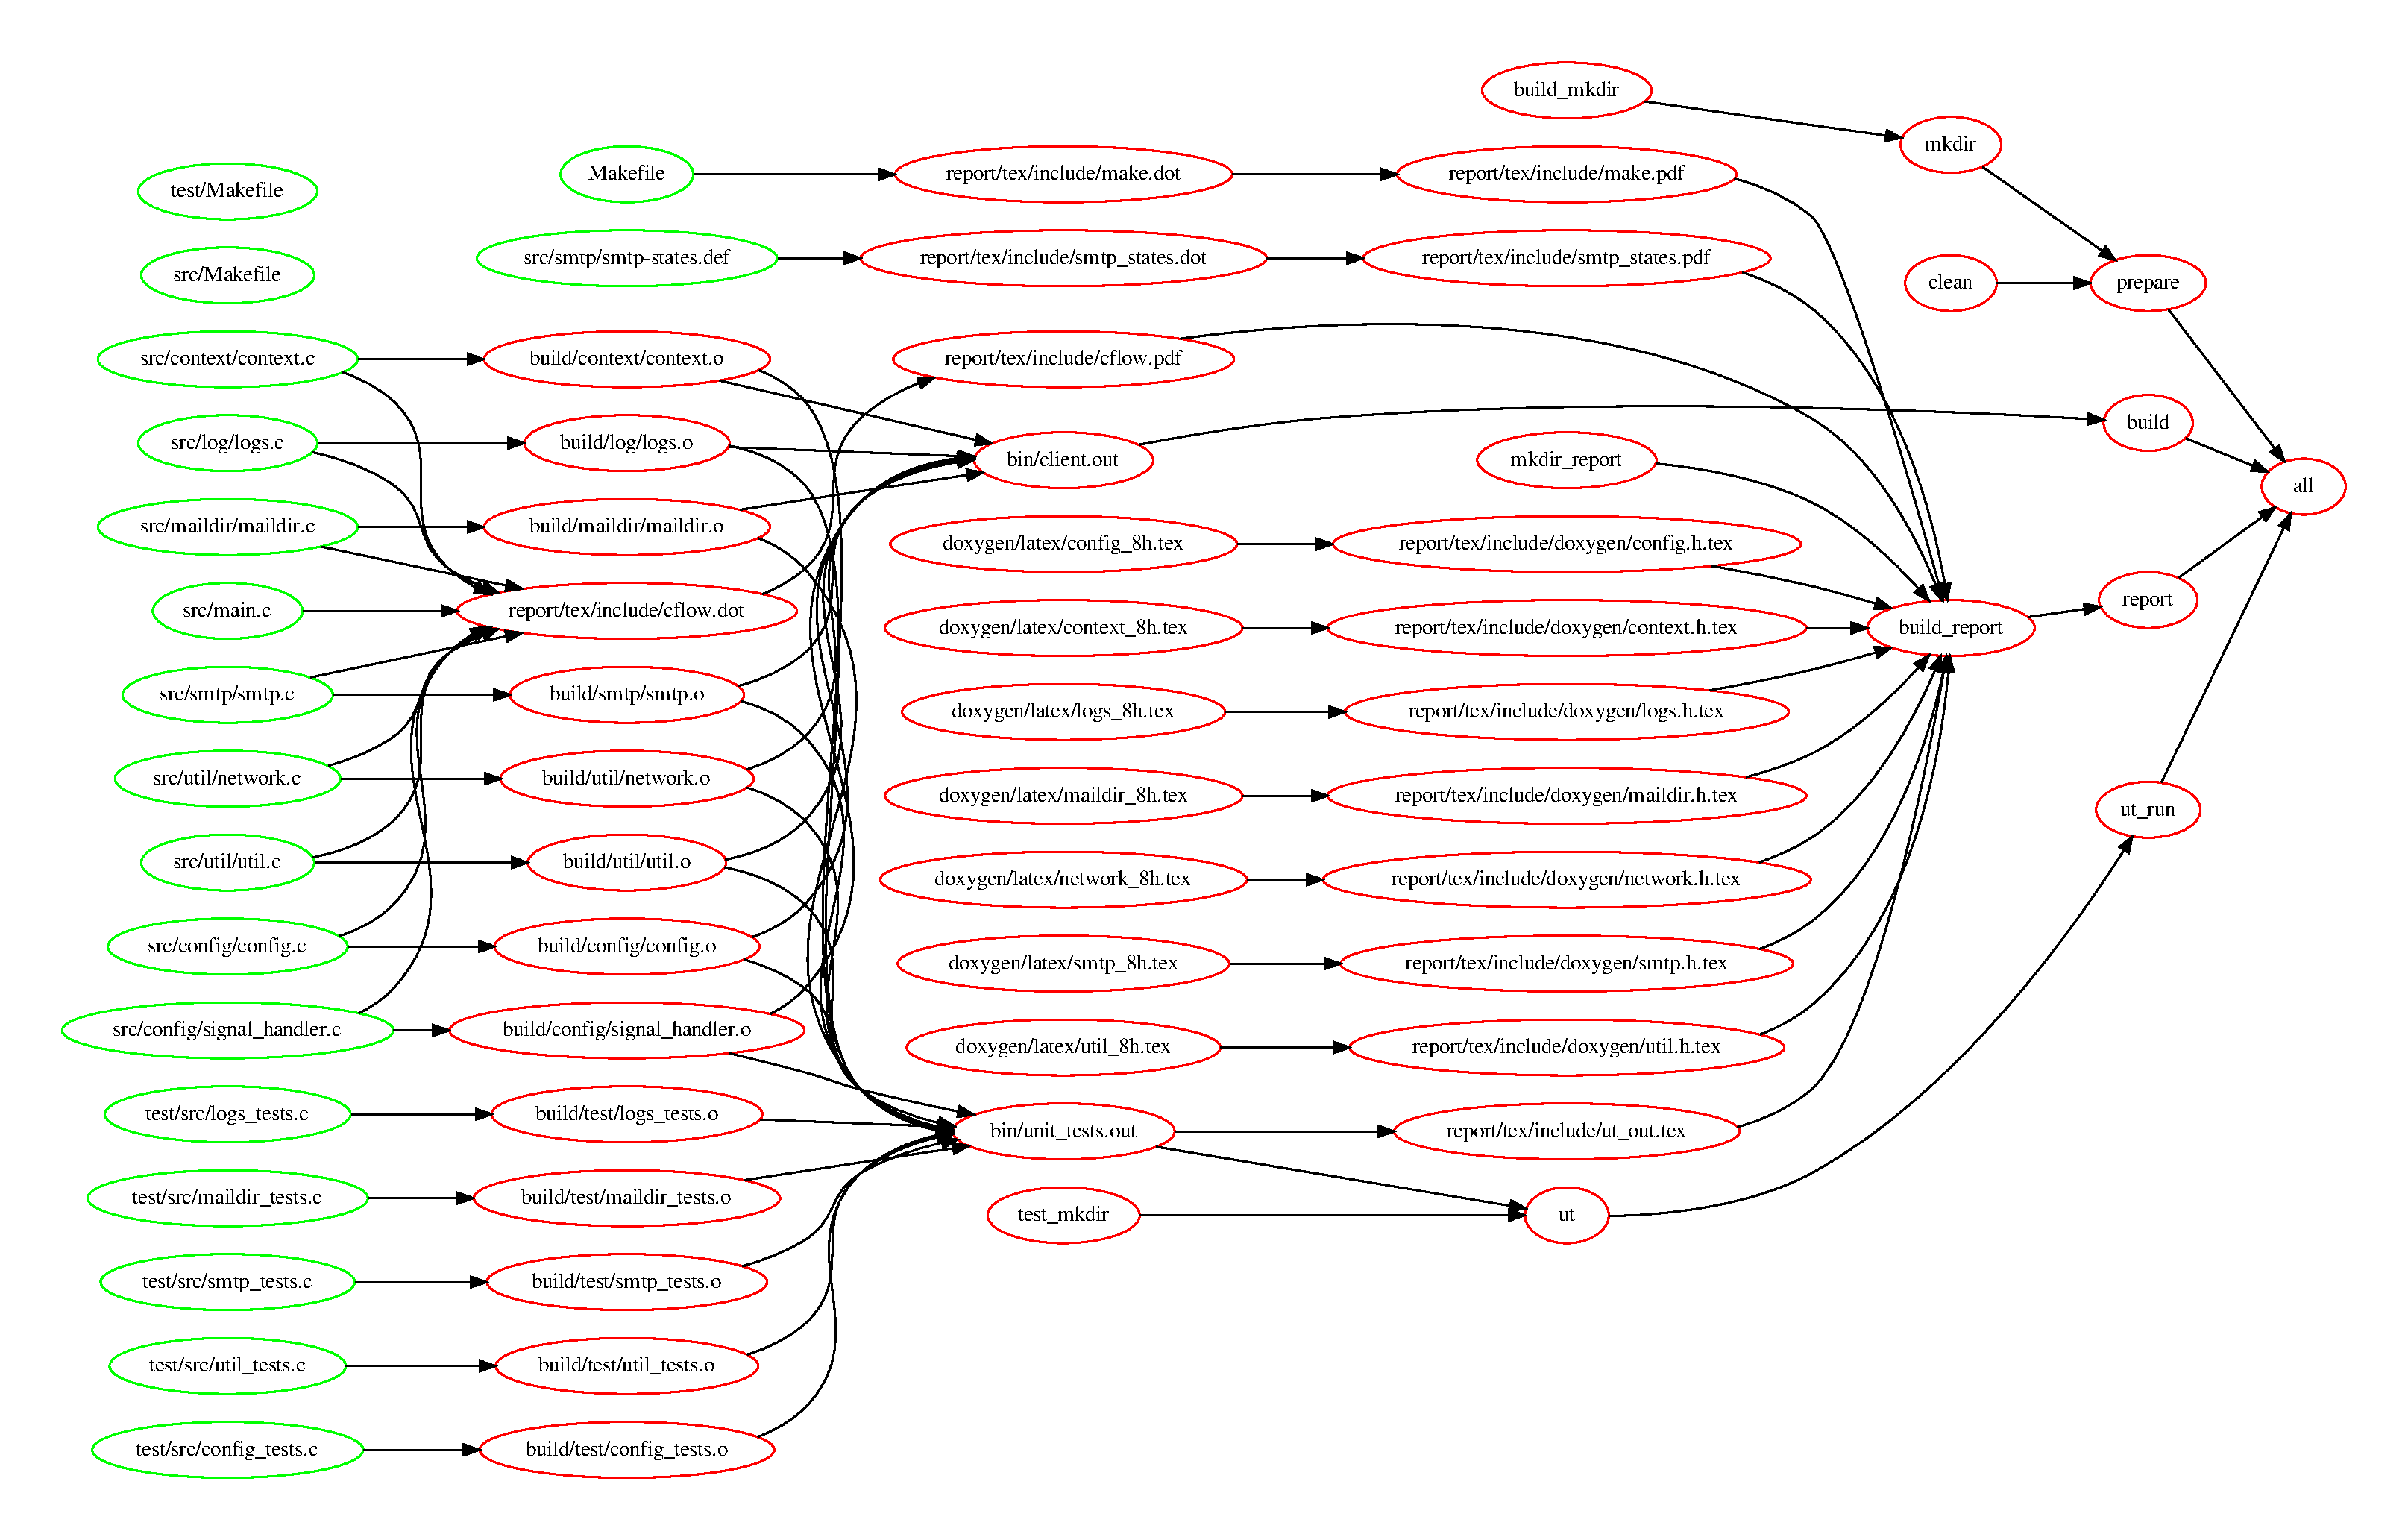
\includegraphics[width=\textwidth]{./include/make.pdf}
	\caption{Структура проекта.}
	\label{fig:makeclient}
	\end{figure}

	Также с помощью утилиты \textbf{cflow} был построен граф вызовов функций (рис. \ref{fig:cflow}), который отражает все взаимосвязи между модулями проекта.
	
	\begin{figure}[H]
	\centering
	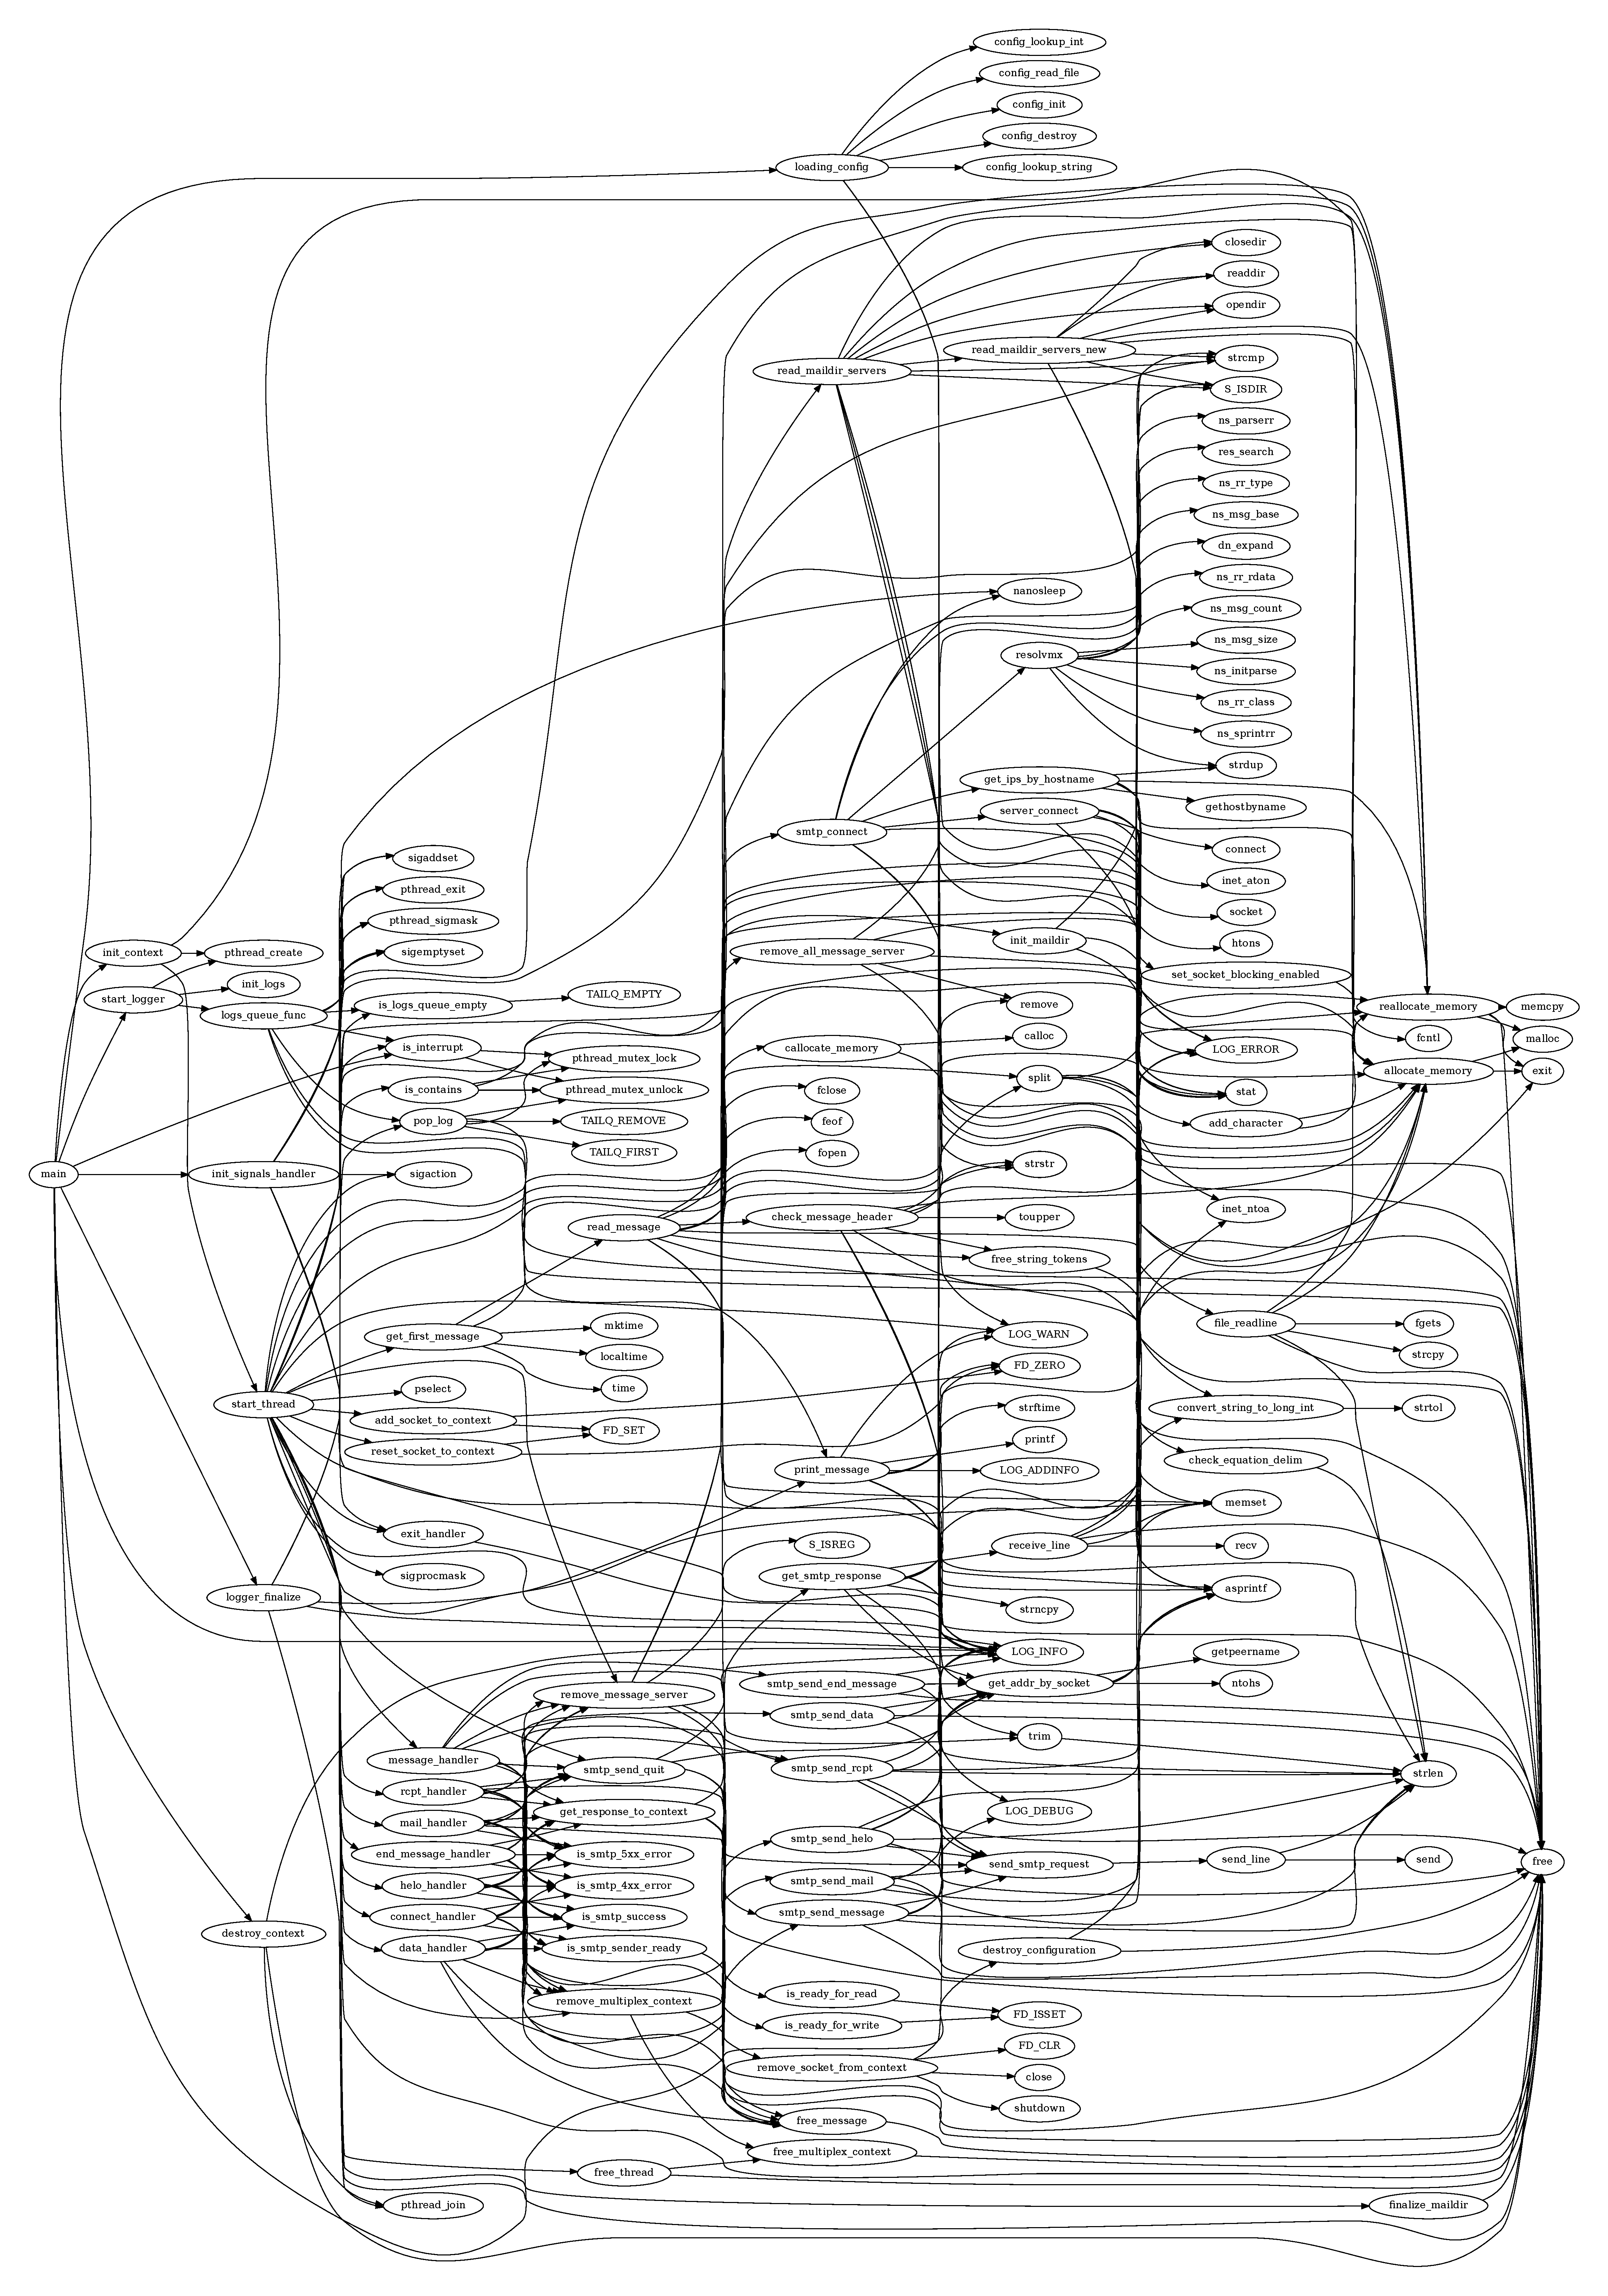
\includegraphics[width=\textwidth]{./include/cflow.pdf}
	\caption{Граф вызовов функций, который реализует всю логику.}
	\label{fig:cflow}
	\end{figure}

	\section{Тестирование}
	
	Для тестирования отдельных модулей клиента были написаны юнит-тесты с использованием библиотеки CUNIT. Ниже представлен результат юнит-тестирования с использованием valgrind. 
	\VerbatimInput{./include/ut_out.tex}
	\VerbatimInput{./include/valgrind_out.tex}

	\section{Основные функции программы}

	Основные функции программы представлены ниже.

	\input{./include/doxygen/config.h.tex}
	\input{./include/doxygen/context.h.tex}
	\input{./include/doxygen/logs.h.tex}   
	\input{./include/doxygen/maildir.h.tex}
	\input{./include/doxygen/smtp.h.tex}
	\input{./include/doxygen/util.h.tex}
	\input{./include/doxygen/network.h.tex}	

	\section{Заключение}
	
	В результате выполнения данной курсовой работы был изучен протокол SMTP. Разработан и реализован SMTP-клиент как часть MTA. Был изучен способ многопоточной обработки с использованием механизма мультиплексирования, когда несколько исходящих соединений обрабатываются в одном потоке исполнения. Разработка SMTP-клиента сопровождалась построением диаграмм, в том числе и конечного автомата для последующей разработке общения SMTP-клиента с удаленным SMTP-сервером. Проведено комплексное тестирование, включающее в себя юнит-тесты и интеграционные тесты в комплексе с ручным тестированием. Также были соблюдены все этапы жизненного цикла разработки ПО, включая в себя автоматизированную сборку проекта с использование CI.
	
	В заключение можно сделать вывод, что все поставленные задачи в рамках курсовой работы по разработке многопоточного SMTP-клиента как части MTA были выполнены.

	\section{Список источников и литературы}
	\begin{enumerate}
		\item RFC.COM.RU. Simple Mail Transfer Protocol [Электронный ресурс]. URL: http://rfc.com.ru/rfc2821.htm (дата обращения 20.12.2020).
		\item Wikipedia.org. SMTP [Электронный ресурс]. URL: https://ru.wikipedia.org/wiki/SMTP (дата обращения 20.12.2020).
		\item CUnit. A unit testing framework for C [Электронный ресурс]. URL: http://cunit.sourceforge.net/ (дата обращения 21.12.2020).
		\item Valgrind. Documentation [Электронный ресурс]. URL: https://www.valgrind.org/docs/manual/index.html (дата обращения 21.12.2020).
		\item Wikibooks.org. LaTeX [Электронный ресурс]. URL: https://ru.wikibooks.org/wiki/LaTeX (дата обращения 21.12.2020).
		\item RSDN. Программирование сокетов в Linux [Электронный ресурс]. URL: https://rsdn.org/article/unix/sockets.xml (дата обращения 21.12.2020).
		\item Хабр. select / poll / epoll: практическая разница [Электронный ресурс]. URL: https://habr.com/ru/company/infopulse/blog/415259/ (дата обращения 19.12.2020).
	\end{enumerate}
	
	\newpage	
\end{document}
